% !TEX root = ../../presentation.tex

\begin{slide}{Model Layer}
\vspace{0.5cm}
\pause

% \begin{tikzpicture}[thick]
%   \tikzset{box/.style={draw, rectangle, text width=1.75cm, text height=0.75cm}}
%
%   % Model
%   \path (0, 0) coordinate (i) node {
\includegraphics[scale=0.1]{cppcon-logo}};
%   \path (2.5, 0) coordinate [box] (E) node {Encoder};
%   \path (4.5, 0) coordinate (z) node {$\mathbf{z}$};
%   \path (6.5, 0) coordinate [box] (D) node {Decoder};
%   \path (9, 0) coordinate (r)
%         node {
\includegraphics[scale=0.1]{cppcon-logo-blurry}};
%
%   % Edges
%   \draw [->, shorten <=0.75cm] (i) -- (E);
%   \draw [->, shorten >=0.25cm] (E) -- (z);
%   \draw [->, shorten <=0.25cm] (z) -- (D);
%   \draw [->, shorten >=0.75cm] (D) -- (r);
%
%   % Label
%   \draw (4.5, -1.2) node {\textbf{Autoencoder}};
% \end{tikzpicture}
% \pause

% \vspace{0.5cm}

\begin{tikzpicture}[thick]
  \tikzset{box/.style={draw, rectangle, text width=1.75cm, text height=0.75cm}}

  % Model
  \path (0, 0) coordinate (z) node {$\mathbf{z}$};
  \path (1.75, 0) coordinate [box] (G) node {Generator};
  \node (f) at (4.25, -0.7) {
\includegraphics[scale=0.075]{bjarne-blurry}};
  \draw [white, rounded corners=6pt, line width=9pt]
      (f.north west) --
      (f.north east) --
      (f.south east) --
      (f.south west) -- cycle;

  \node (r) at (4.25, +0.7) {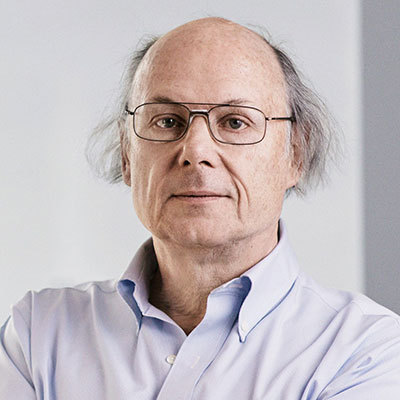
\includegraphics[scale=0.075]{bjarne}};
  \draw [white, rounded corners=6pt, line width=9pt]
      (r.north west) --
      (r.north east) --
      (r.south east) --
      (r.south west) -- cycle;

  \path (7.25, 0) coordinate [box, text width=2.2cm] (D) node {Discriminator};
  \path (5.7, 0) coordinate (_);
  \path (9.75, 0) coordinate (P) node {$\mathbf{P(\text{real})}$};

  % Edges
  \draw [->, shorten <=0.25cm] (z) -- (G);
  \draw [->] (G) edge [out=0, in=180] (f);
  \draw (f) edge [out=0, in=180] (_);
  \draw (r) edge [out=0, in=180] (_);
  \draw [->] (_) -- (D);
  \draw [->, shorten >=0.75cm] (D) -- (P);

  % Label
  \draw (5.5, -2.4) node {\textbf{Generative Adversarial Network (GAN)}};
\end{tikzpicture}
\end{slide}

% \begin{slide}{Generative Adversarial Networks}
% $$
% \underbrace{\mathbf{z} \sim P_{\text{noise}}(\mathbf{z})}_\text{Noise}
% \hspace{0.4cm}
% \underbrace{\mathbf{x} \sim P_{\text{data}}(\mathbf{x})}_\text{Real Images}
% $$
% \vspace{0.1cm}
% $$
% \underbrace{G(\mathbf{z})}_\text{Fake Images}
% \hspace{0.4cm}
% \underbrace{D(\mathbf{x})}_\text{Probability of Being Real}
% $$
%
% \only<2>{
% $$
% \frac{%
% \int_{-\infty}^\infty
%     \hat f(\xi)\,e^{2 \pi i \xi x}
%     \,d\xi + \sum_{n=0}^\infty \frac{f^{(n)}(a)}{n!} + {e^2 \brace \pi}
% }{%
% \frac{1}{\sqrt{2\pi\hbar}}\int_{\text{all space}}e^{-i\mathbf{p}\cdot r/\hbar}\Psi(\mathbf{r}, s_z, t)d^3\mathbf{r} - \frac{1}{\sqrt{2\pi\sigma^2}} \cdot e^{-\frac{(x - \mu)^2}{2\sigma^2}}
% }
% $$
% }
%
% \only<3->{
% $$
% \min_G \max_D\, \log(D(\mathbf{x})) + \log(1 - D(G(\mathbf{z})))
% $$
% }
% \end{slide}

\begin{slide}{Generative Adversarial Networks}
  % 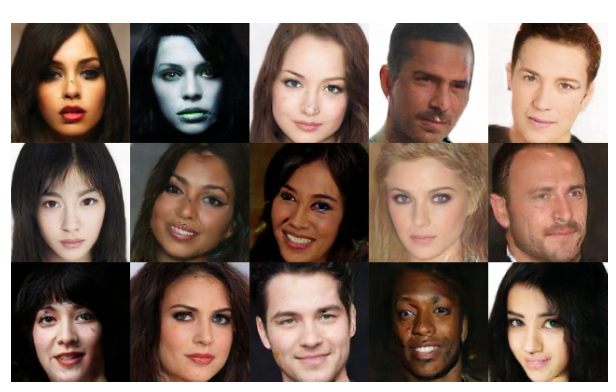
\includegraphics[scale=0.45]{began-faces}
  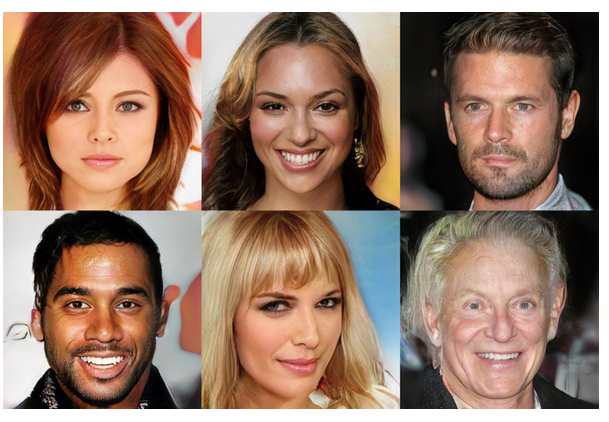
\includegraphics[scale=0.4]{progressive-gan-faces}

  \vspace{0.1cm}
  \begin{flushleft}
    \scriptsize
    % BEGAN: Berthelot et al. (2017)
    Progressive GAN: Karras et al. (2017)
  \end{flushleft}
\end{slide}

% \begin{slide}{Generative Adversarial Networks}
%   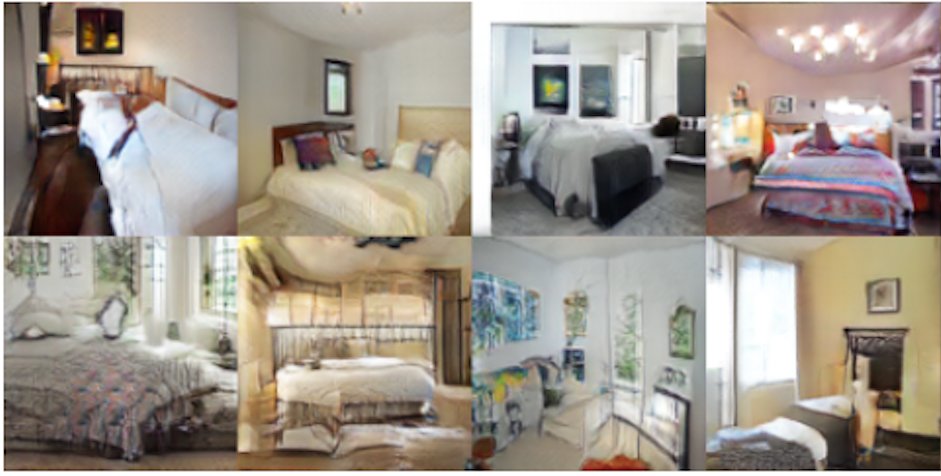
\includegraphics[scale=0.3]{bedrooms}
%
%   \scriptsize
%   LSGAN: Mao et al. (2016)
% \end{slide}

\begin{slide}{Generative Adversarial Networks}
  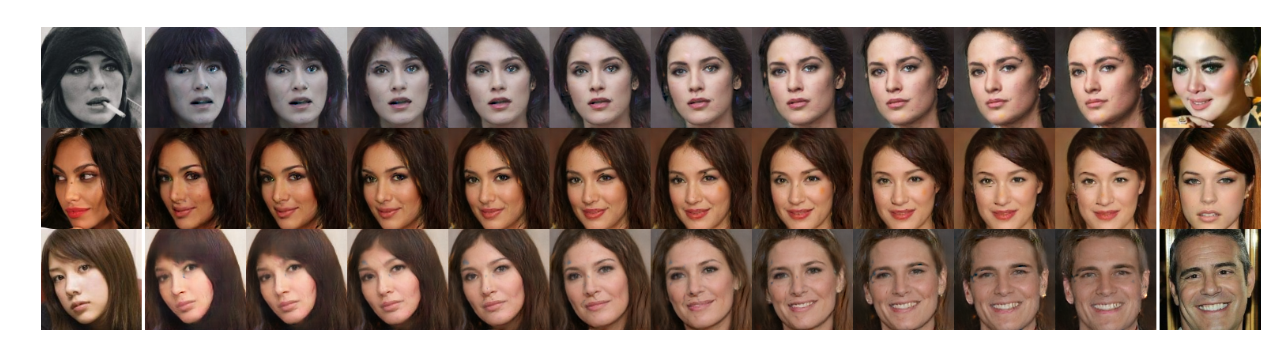
\includegraphics[scale=0.235]{face-interpolations}

  \vspace{0.1cm}
  \begin{flushleft}
    \scriptsize
    BEGAN: Berthelot et al. (2017)
  \end{flushleft}
\end{slide}

% \begin{slide}{Generative Adversarial Networks}
%   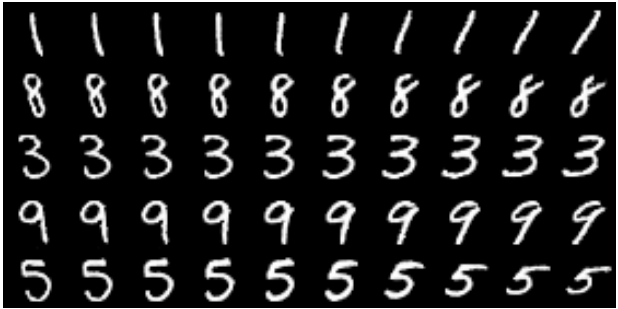
\includegraphics[scale=0.3]{mnist1}
%
%   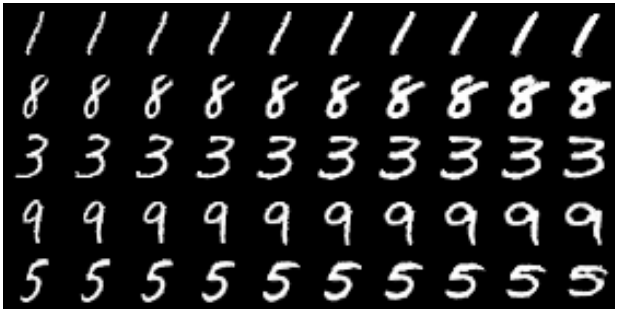
\includegraphics[scale=0.3]{mnist2}
%
%   \scriptsize
%   InfoGAN: Chen et al. (2016)
% \end{slide}
